\documentclass[svgnames,11pt]{beamer}
\input{/home/tof/Documents/Cozy/latex-include/preambule_commun.tex}
\input{/home/tof/Documents/Cozy/latex-include/preambule_beamer.tex}
%\usepackage{pgfpages} \setbeameroption{show notes on second screen=left}
\author[]{Christophe Viroulaud}
\title{Processus et temps partagé}
\date{\framebox{\textbf{Archi 08}}}
%\logo{}
\institute{Terminale - NSI}

\begin{document}
\begin{frame}
    \titlepage
\end{frame}
\begin{frame}
    \frametitle{}

    Dans les années 60, \textbf{Multics} est un des premiers systèmes d'exploitation avec:
    \begin{itemize}
        \item système de fichier hiérarchique,
        \item temps partagé,
        \item multitâche préemptif,
        \item multi-utilisateur.
    \end{itemize}
    \note[item]{préemptif: capacité d'un système d'exploitation à exécuter ou arrêter une tâche planifiée en cours.}
    \note[item]{fin 70: unix (Thomson, Ritchie) pour créer un système plus simple}
\end{frame}
\begin{frame}
    \frametitle{}

    \begin{center}
        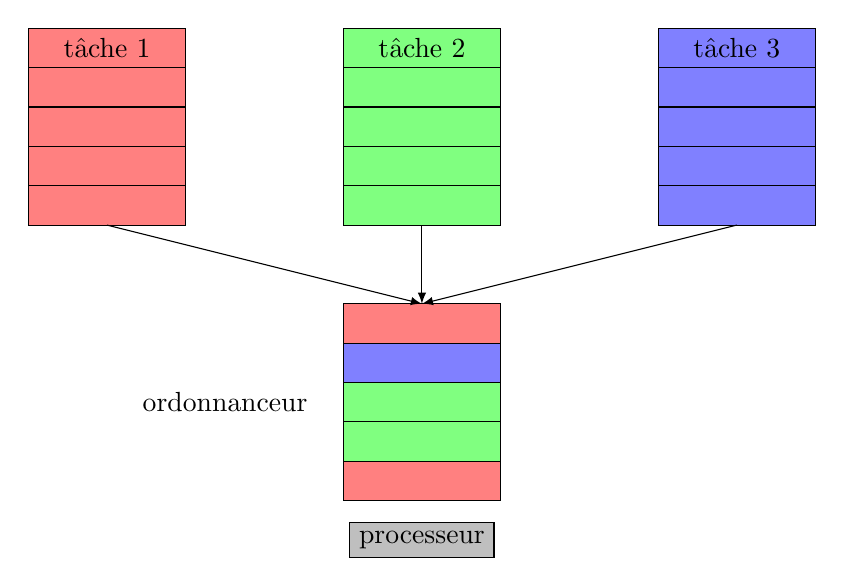
\begin{tikzpicture}
            \foreach \c/\x/\t in {red/0/tâche 1, green/4/tâche 2, blue/8/tâche 3}{
                    \fill[color=\c!50] (0+\x,0) -- (2+\x,0) -- (2+\x,2.5) -- (0+\x,2.5) -- cycle;
                    \draw (0+\x,0) grid[xstep=2cm,ystep=0.5cm] (2+\x,2.5);
                    \node at(1+\x,2.25) {\t};
                }

            \foreach \c/\y in {red/0, green/0.5, green/1, blue/1.5,red/2}{
                    \fill[color=\c!50] (4,-3.5+\y) -- (6,-3.5+\y) -- (6,-3+\y) -- (4,-3+\y) -- cycle;
                }
            \draw (4,-3.5) grid[xstep=2cm,ystep=0.5cm] (6,-1);
            \node[draw,fill=gray!50]at(5,-4){processeur};
            \node at(2.5,-2.25){ordonnanceur};
            \draw[->,>=latex] (1,0) -- (5,-1);
            \draw[->,>=latex] (5,0) -- (5,-1);
            \draw[->,>=latex] (9,0) -- (5,-1);
        \end{tikzpicture}
        \captionof{figure}{Système mono-processeur}
    \end{center}
    \note{tâches créées par utilisateur}
\end{frame}

\begin{frame}
    \frametitle{}

    \begin{center}
        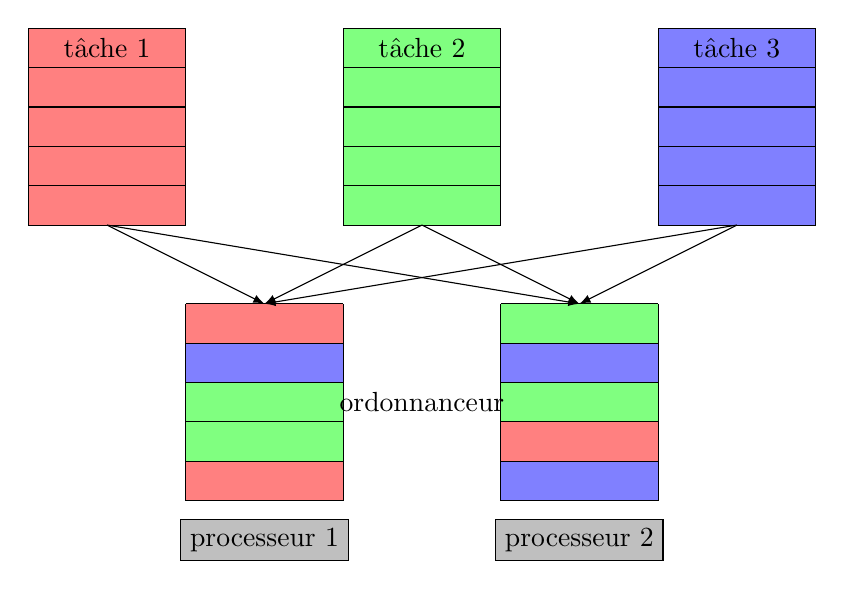
\begin{tikzpicture}
            \foreach \c/\x/\t in {red/0/tâche 1, green/4/tâche 2, blue/8/tâche 3}{
                    \fill[color=\c!50] (0+\x,0) -- (2+\x,0) -- (2+\x,2.5) -- (0+\x,2.5) -- cycle;
                    \draw (0+\x,0) grid[xstep=2cm,ystep=0.5cm] (2+\x,2.5);
                    \node at(1+\x,2.25) {\t};
                }

            \foreach \c/\y in {red/0, green/0.5, green/1, blue/1.5,red/2}{
                    \fill[color=\c!50] (2,-3.5+\y) -- (4,-3.5+\y) -- (4,-3+\y) -- (2,-3+\y) -- cycle;
                }
            \draw (2,-3.5) grid[xstep=2cm,ystep=0.5cm] (4,-1);
            \node[draw,fill=gray!50]at(3,-4){processeur 1};

            \foreach \c/\y in {blue/0, red/0.5, green/1, blue/1.5,green/2}{
                    \fill[color=\c!50] (6,-3.5+\y) -- (8,-3.5+\y) -- (8,-3+\y) -- (6,-3+\y) -- cycle;
                }
            \draw (6,-3.5) grid[xstep=2cm,ystep=0.5cm] (8,-1);
            \node[draw,fill=gray!50]at(7,-4){processeur 2};

            \node at(5,-2.25){ordonnanceur};
            \draw[->,>=latex] (1,0) -- (3,-1);
            \draw[->,>=latex] (1,0) -- (7,-1);
            \draw[->,>=latex] (5,0) -- (3,-1);
            \draw[->,>=latex] (5,0) -- (7,-1);

            \draw[->,>=latex] (9,0) -- (3,-1);
            \draw[->,>=latex] (9,0) -- (7,-1);
        \end{tikzpicture}
        \captionof{figure}{Système multi-processeurs}
    \end{center}
    \note{tâches créées par utilisateur}
\end{frame}
\begin{frame}
    \frametitle{}

    \begin{activite}
        Identifier les problèmes éventuels dans les deux types d'architectures.
    \end{activite}

\end{frame}
\begin{frame}
    \frametitle{Correction}

    \begin{itemize}
        \item Deux tâches ont besoin d'utiliser la même ressource.
        \item Une tâche a besoin de réaliser certaines actions dans un ordre précis.
    \end{itemize}
    \note{exemple: Imaginons le cas où les tâches 1 et 2 ont besoin d'utiliser la même ressource (webcam)}
\end{frame}
\begin{frame}
    \frametitle{}

    \begin{framed}
        \centering Comment ordonner les processus pour minimiser les erreurs d'exécution?
    \end{framed}

\end{frame}
\section{Parallélisme}
\subsection{Programmation séquentielle}
\begin{frame}[fragile]
    \frametitle{Programmation séquentielle}

    \begin{center}
        \begin{lstlisting}[language=Python , basicstyle=\ttfamily\small, xleftmargin=2em, xrightmargin=2em]
def f1():
    for _ in range(5):
        print("appel 1")

def f2():
    for _ in range(5):
        print("appel 2")

f1()
f2()
\end{lstlisting}
        \captionof{code}{}
        \label{seq}
    \end{center}
    \begin{activite}
        Exécuter le code \ref{seq}.
    \end{activite}
\end{frame}
\begin{frame}[fragile]
    \frametitle{}

    \begin{center}
        \begin{lstlisting}[language=Python , basicstyle=\ttfamily\small, xleftmargin=2em, xrightmargin=2em]
appel 1
appel 1
appel 1
appel 1
appel 1
appel 2
appel 2
appel 2
appel 2
appel 2
\end{lstlisting}
        \captionof{code}{L'interpréteur exécute les lignes de code séquentiellement.}
    \end{center}

\end{frame}
\subsection{Programmation en parallèle}
\begin{frame}
    \frametitle{Programmation en parallèle - notion de \textbf{thread}}

    Les ordinateurs possèdent maintenant plusieurs processeurs. Il semble alors pertinent de partager les tâches pour accélérer l'exécution des processus.

\end{frame}
\begin{frame}
    \frametitle{}

    \begin{center}
        Un thread est un processus qui va s'exécuter simultanément avec d'autres thread en partageant l'espace des données.
    \end{center}

\end{frame}
\begin{frame}[fragile]
    \frametitle{}

    \begin{center}
        \begin{lstlisting}[language=Python , basicstyle=\ttfamily\small, xleftmargin=2em, xrightmargin=2em]
from threading import Thread
from time import sleep

def f1():
    for _ in range(5):
        print("appel 1")
        sleep(0.01)

def f2():
    for _ in range(5):
        print("appel 2")
        sleep(0.01)

p1 = Thread(target=f1)
p2 = Thread(target=f2)
p1.start()
p2.start()
\end{lstlisting}
        \captionof{code}{Deux thread en parallèle}
        \label{thread}
    \end{center}
    \note{sleep pour ralentir un peu sinon f1 s'exécuterait tout d'un coup}
    \begin{activite}
        Simuler l'exécution de deux processus fonctionnant en parallèle à l'aide du code \ref{thread}.
    \end{activite}
\end{frame}
\begin{frame}[fragile]
    \frametitle{}

    \begin{center}
        \begin{lstlisting}[language=Python , basicstyle=\ttfamily\small, xleftmargin=2em, xrightmargin=2em]
appel 1
appel 2
appel 1
appel 1
appel 2
appel 1
appel 2
appel 1
appel 2
appel 2
\end{lstlisting}
        \captionof{code}{L'interpréteur exécute les lignes de code séquentiellement.}
    \end{center}
    \note{relancer plusieurs fois; sleep ×10 ou ÷10 si marche pas}
\end{frame}
\subsection{Répartition des tâches: solution à risques}
\begin{frame}[fragile]
    \frametitle{Répartition des tâches: solution à risques}

    \begin{center}
        \begin{lstlisting}[language=Python , basicstyle=\ttfamily\small, xleftmargin=1em, xrightmargin=0em]
from time import sleep
INTERMEDIAIRE = 0

def calcul():
    global INTERMEDIAIRE
    print("section non critique 1")
    for c in range(400):
        temp = INTERMEDIAIRE
        # simule un traitement long
        sleep(0.000000001)        
        INTERMEDIAIRE = temp + 1
    print("section non critique 2")

calcul()
print(INTERMEDIAIRE)
\end{lstlisting}
        \captionof{code}{Simuler un calcul (séquentiel) long}
        \label{simul1}
    \end{center}

\end{frame}
\begin{frame}
    \frametitle{}

    \begin{activite}
        \begin{enumerate}
            \item Télécharger et extraire le dossier compressé \textbf{\texttt{processus-prog-concurrente-annexe}}.
            \item Ouvrir le fichier \textbf{\texttt{compteur\_sequentielle.py}} qui simule un calcul long.
        \end{enumerate}
    \end{activite}
    \begin{aretenir}[Commentaire]
        \begin{itemize}
            \item La variable globale \textbf{\texttt{INTERMEDIAIRE}} simule un résultat qui évolue quand le traitement long est terminé.
            \item La boucle est la \textbf{section critique} du calcul.
        \end{itemize}
    \end{aretenir}
\end{frame}
\begin{frame}
    \frametitle{}

    \begin{center}
        La variable globale \textbf{\texttt{INTERMEDIAIRE}} contient \textbf{\texttt{400}} à la fin de l'exécution.
    \end{center}

\end{frame}
\begin{frame}[fragile]
    \frametitle{Partager les traitements longs}

    \begin{center}
        \begin{lstlisting}[language=Python , basicstyle=\ttfamily\small, xleftmargin=2em, xrightmargin=2em]
tab_threads = []
# Lance en parallèle 4 exécutions de calcul
for i in range(4):  
    p = Thread(target=calcul)
    p.start() 
    tab_threads.append(p)
\end{lstlisting}
        \captionof{code}{Exécution en parallèle}
        \label{simul2}
    \end{center}
    Le code \ref{simul2} lance quatre processus en parallèle pour réaliser les calculs longs.

\end{frame}
\begin{frame}
    \frametitle{}

    \begin{activite}
        \begin{enumerate}
            \item Ouvrir le fichier \textbf{\texttt{compteur\_thread.py}}.
            \item Dans la boucle de la fonction, remarquer que le nombre d'itérations a été divisé par 4.
            \item Exécuter le programme.
            \item Qu'observe-t-on? Comment expliquer ce résultat?
        \end{enumerate}
    \end{activite}

\end{frame}
\begin{frame}
    \frametitle{Correction}

    \begin{itemize}
        \item La variable \textbf{\texttt{temp}} est locale: elle dépend de chaque appel de la fonction.
        \item La variable \textbf{\texttt{INTERMEDIAIRE}} est globale: elle est \emph{partagée} entre les appels.
    \end{itemize}

\end{frame}
\begin{frame}
    \frametitle{}

    Un scénario possible:
    \begin{itemize}
        \item \textbf{\texttt{thread 1:}} \textbf{\texttt{$temp_1=10$}}
        \item \textbf{\texttt{thread 2:}} \textbf{\texttt{$temp_2=10$}}
        \item \textbf{\texttt{thread 3:}} \textbf{\texttt{$temp_3=10$}}
        \item \textbf{\texttt{fin thread 1:}} \textbf{\texttt{$INTERMEDIAIRE=temp_1+1=11$}}
        \item \textbf{\texttt{fin thread 2:}} \textbf{\texttt{$INTERMEDIAIRE=temp_2+1=11$}}
        \item \textbf{\texttt{thread 4:}} \textbf{\texttt{$temp_4=11$}}
        \item \textbf{\texttt{fin thread 3:}} \textbf{\texttt{$temp_3=11$}}
        \item \textbf{\texttt{fin thread 4:}} \textbf{\texttt{$INTERMEDIAIRE=temp_4+1=12$}}
    \end{itemize}
    \begin{center}
        \textbf{\texttt{INTERMEDIAIRE}} vaut 12 alors qu'il y a eu 4 appels à la fonction \textbf{\texttt{calcul}}.
    \end{center}
\end{frame}
\begin{frame}
    \frametitle{}

    \begin{aretenir}[Observation]
        On ne maîtrise pas l'ordre d'exécution des threads.
    \end{aretenir}

\end{frame}
\begin{frame}
    \frametitle{Contrôler la \emph{section critique}}

    \begin{center}
        Il est possible de bloquer l'exécution d'un thread pour l'obliger à attendre la fin d'une \textbf{section critique}.
    \end{center}

\end{frame}
\begin{frame}
    \frametitle{}

    \begin{activite}
        \begin{enumerate}
            \item Ouvrir le fichier \textbf{\texttt{compteur\_verrou.py}}.
            \item Interpréter le rôle du verrou.
        \end{enumerate}
    \end{activite}

\end{frame}
\begin{frame}
    \frametitle{}

    \begin{itemize}
        \item \textbf{\texttt{acquire}} prend le verrou ou attend qu'il se libère.
        \item \textbf{\texttt{release}} libère le verrou.
    \end{itemize}
    \begin{center}
        \textbf{\texttt{INTERMEDIAIRE}} vaut 100 à la fin de l'exécution du programme.
    \end{center}
\end{frame}
\section{Interblocage}
\subsection{Exemple de situation}
\begin{frame}
    \frametitle{Interblocage - exemple de situation}

    En 1997, la mission Mars Pathfinder rencontre un problème alors que le robot est déjà sur Mars. Après un certain temps, des données sont systématiquement perdues. Les ingénieurs découvrent alors un bug lié à la synchronisation de plusieurs tâches.
    \begin{center}
        \centering
        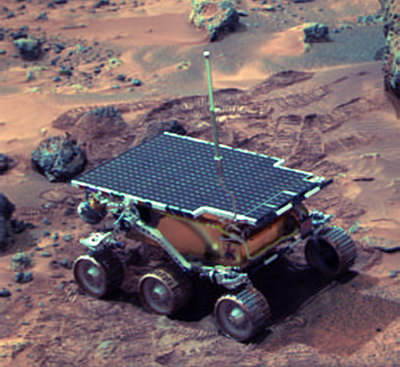
\includegraphics[width=4cm]{ressources/pathfinder.jpg}
        \captionof{figure}{Robot Pathfinder}
        \label{IMG}
    \end{center}

\end{frame}
\begin{frame}
    \frametitle{}

    Considérons un robot qui possède 3 ressources:
    \begin{itemize}
        \item des \textbf{moteurs} qui lui permettent de se déplacer,
        \item une liaison \textbf{wifi} qui lui permet de communiquer,
        \item une \textbf{caméra} qui filme son environnement.

    \end{itemize}
    \vspace{1.5cm}
    Il peut réaliser 3 tâches:
    \begin{itemize}
        \item le \textbf{pilotage manuel} qui reçoit les ordres par le wifi et actionne les moteurs,
        \item envoie le \textbf{flux vidéo} via la liaison wifi,
        \item fait un \textbf{autotest} matériel, hors liaison wifi.

    \end{itemize}
\end{frame}
\begin{frame}
    \frametitle{}

    \begin{center}
        \begin{tabular}{|*{3}{c|}}
            \hline
            \textbf{pilotage manuel} & \textbf{flux vidéo} & \textbf{autotest} \\
            \hline
            Demande moteurs          & Demande wifi        & Demande caméra    \\
            Demande wifi             & Demande caméra      & Demande moteurs   \\
            Libère moteurs           & Libère wifi         & Libère caméra     \\
            Libère wifi              & Libère caméra       & Libère moteurs    \\
            \hline
        \end{tabular}
        \captionof{table}{Détails des tâches}
    \end{center}

\end{frame}
\begin{frame}
    \frametitle{}

    Imaginons le scénario:
    \begin{itemize}
        \item Le pilotage manuel demande les moteurs et les obtient.
        \item Le flux vidéo demande le wifi et l'obtient.
        \item L'autotest demande la caméra et l'obtient.
        \item Le pilotage manuel demande le wifi mais doit attendre que le flux vidéo le libère.
        \item Le flux vidéo demande la caméra mais doit attendre que l'autotest la libère.
        \item L'autotest demande les moteurs mais doit attendre que le pilotage manuel les libère.
    \end{itemize}
    \begin{center}
        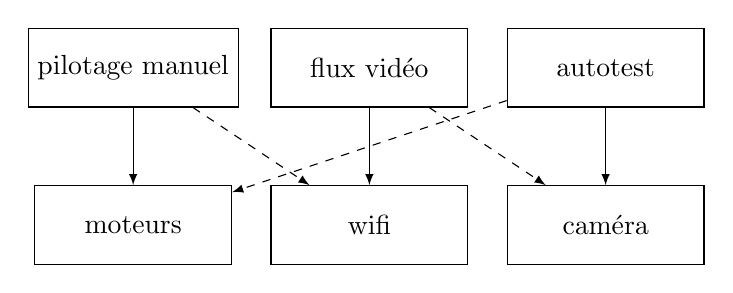
\begin{tikzpicture}
            \foreach \i/\n/\x/\y in {0/pilotage manuel/0/0,
                    1/flux vidéo/3/0, 2/autotest/6/0, 3/moteurs/0/-2,
                    4/wifi/3/-2, 5/caméra/6/-2}{
                    \node[draw, minimum width=2.5cm, minimum height=1cm] (\i) at (\x,\y) {\n};
                }
            \draw[->,>=latex] (0) -- (3);
            \draw[->,>=latex] (1) -- (4);
            \draw[->,>=latex] (2) -- (5);
            \draw[->,>=latex,dashed] (0) -- (4);
            \draw[->,>=latex,dashed] (1) -- (5);
            \draw[->,>=latex,dashed] (2) -- (3);
        \end{tikzpicture}
    \end{center}
\end{frame}
\begin{frame}
    \frametitle{}

    \begin{activite}
        \begin{enumerate}
            \item Ouvrir le fichier \textbf{\texttt{interblocage.py}}.
            \item Observer le cas d'interblocage. Appuyer deux fois sur \textbf{\texttt{ctrl+C}} pour tuer les processus.
        \end{enumerate}
    \end{activite}

\end{frame}
\subsection{Conditions d'interblocage}
\begin{frame}
    \frametitle{Conditions d'interblocage}

    L'interblocage est le grand danger de la programmation concurrente. Il existe quatre conditions nécessaires à la présence d'un interblocage, décrites par Edward Grady Coffman en 1971:
    \begin{itemize}
        \item<1-> \textbf{Exclusion mutuelle:} au moins une ressource doit être en accès exclusif.
        \item<2-> \textbf{Rétention et attente:} un processus détient une ressource et demande une autre ressource détenue par un autre processus.
        \item<3-> \textbf{Non préemption:} une ressource détenue par un processus ne peut être récupérée de force (\emph{préemptée}) par un autre processus.
        \item<4-> \textbf{Attente circulaire:} chaque processus attend une ressource détenue par un des autres.
    \end{itemize}

\end{frame}
\subsection{Traitement de l'interblocage}
\begin{frame}
    \frametitle{Traitement de l'interblocage}

    Sans rentrer dans le détail, nous pouvons citer les politiques mises en place pour traiter l'interblocage:
    \begin{itemize}
        \item<1-> \textbf{Politique de guérison:} le système maintient un état permanent des demandes de ressources et résout les éventuels interblocages en tuant un processus.
        \item<2-> \textbf{Politique de prévention:} le système fait en sorte que les quatre conditions ne soient jamais réunis. Par exemple, ne jamais donner une ressource si elle est déjà utilisée par un autre processus.
        \item<3-> \textbf{Politique de l'évitement:} à chaque demande de ressource, le système vérifie si cela peut causer un interblocage. Si tel est le cas, l'allocation est retardée.
        \item<4-> \textbf{Politique de l'autruche:} on ne s'en occupe pas, et on se contente de redémarrer la machine quand trop de processus sont en interblocage. Les trois autres politiques étant très coûteuses cette solution n'est finalement pas si farfelue.
    \end{itemize}

\end{frame}
\begin{frame}
    \frametitle{Bibliographie}

    \begin{itemize}
        \item \url{http://y.legouzouguec.free.fr}
        \item \url{http://lycee.educinfo.org/index.php?page=introduction&activite=processus}
    \end{itemize}

\end{frame}
\end{document}